\section{Cavern $\gamma$ Generator}
\label{sec:cavern_gamma_generator}

\par
Although the LZ detector has been constructed underground to limit cosmic radiation, it does come with a drawback of being in a mine with a non-negligibly radioactive rock and the shotcreat and gravel within the David Cavern.
LZ is not unique in this, it is a problem highlighted in a number of other underground experiments \cite{cavern_gamma_annual_modulation_CoGeNT_ref, cavern_gammas_in_Soudan_mine_ref}, with an annual modulation mimicking dark matter potentially seen in \cite{cavern_gamma_annual_modulation_CoGeNT_ref}.
The rate of this has been measured and can be attributed to the shotcreat and gravel \cite{LZ_Gamma_Ray_Background_ref}. 
One of the most significant sources of background come not from any internal component but rather from $^{238}U$, $^{232}Th$ and $^{40}K$ decays from the cavern in which the LZ detector exists \cite{LZ_Gamma_Ray_Background_ref}.
However, this is a computationally intensive process to simulation $\gamma$'s where the majority will not reach the actual detector.
To compensate, a generator for these $\gamma$'s was created - and originally described in \cite{rg_generator_ref} but summarised below.
The generator is a created by performing simulations of the decay chains originating in the shotcreat and gravel.
The $\gamma$'s which reach a pre-defined surface are saved.
A second stage simulation is then performed where each of the saved $\gamma$'s is generated a number of times and then saved at another pre-defined surface.
This boost occurs a number of times, until a generator surface.
When subsequent simulations are performed, these saved $\gamma$'s are randomly sampled. 

\par
In order to perform the For the creation of the generator additional cavern properties are added to the simulation.
Namely; a steel pyramid and gravel beneath the water tank, and a layer of shotcreat.
These adaptions are shown in Figure \ref{fig:Cavern_Geometry}.

\begin{figure}[!htbp]
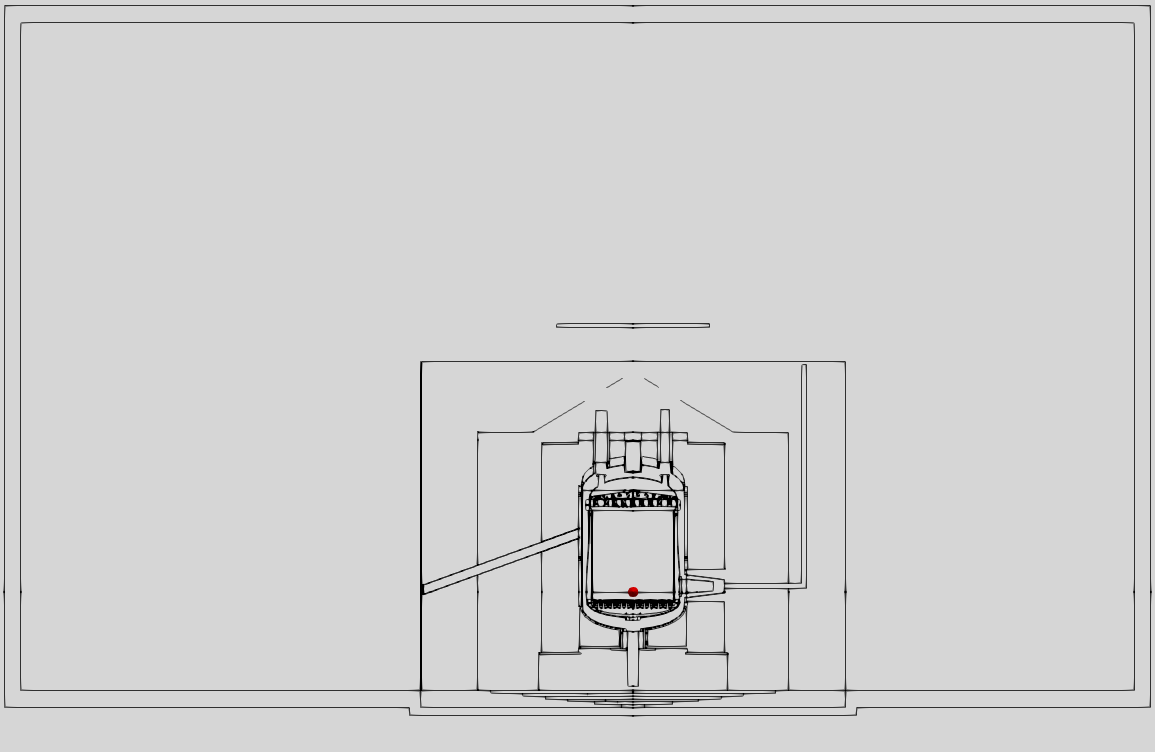
\includegraphics[width=\textwidth]{Figures/Simulations/cavern_geometry_2.png}
\centering
\caption{LZ detector geometry slice with additional cavern geometry. OD PMTs are not seen present as they do not lie in this plane. The red dot marks (0,0,0).}
\label{fig:Cavern_Geometry}
\end{figure}

\par
Although as mentioned in \cite{scotthaselschwardt_thesis_ref}, a generator for the Davis Cavern $\gamma$'s existed, it had a number of flaws.
Firstly, no $\gamma$ below 2MeV was saved.
This meant that $^{40}K$ was not included and so the resultant expected rates being lower than expected.
Additionally, the generator was created using a version of GEANT4 which the rest of the simulation chain had moved on from; GEANT4.9.5 to GEANT4.10.3.p02. 
This motivated the creation of a new generator.

\par
The parameters of the new generator are shown in Table \ref{tab:cavern_gamma_generator_parameters} and a comparison of the energy distribution of the old and new generators is shown in Figure \ref{fig:cavern_gamma_energy_distribution}.
Although it can be seen that the previous generators had a maximum $\gamma$ energy of 10MeV, it also highlights a significant change between GEANT4.9.5 and GEANT4.10.3.p02.
That is, an increased rate above 9MeV.
These $\gamma$'s are predominately from ($\alpha$,$\gamma$) reactions such as $O + \alpha \to Ne + \gamma$.
These are of particular concern as they have the potential to mimic dark matter.
Conversely, they may produce large signals in the OD which would trigger a veto, reducing the detector livetime.
Since this version of GEANT4, there have been new studies of the ($\alpha$,$\gamma$) cross-section in other underground laboratories, such as in \cite{cavern_gammas_in_Soudan_mine_ref}.
Generally, very little attention has been given to ($\alpha$,$\gamma$) rates, and so it is possible that the observed rate may differ significantly from that shown here as although in Figure \ref{fig:cavern_gamma_energy_distribution} the largest difference is at higher energy $\gamma$'s, as was shown in the Sudan Mine \cite{cavern_gammas_in_Soudan_mine_ref}, the rate of sub-6MeV $\gamma$'s may also change significantly. 

\par
The livetime ($l$) for a simulation can be determined then by $l_{\text{simulation}} = \frac{\text{n.} \gamma_{\text{simulated}}}{\text{n.} \gamma_{\text{generator}}} * \text{l}_{\text{generator}}$
In short, this means that every $\gamma$ in the generator represents roughly 130000 decays from the rock, and so is a significant computational saving.


\begin{table}[!htbp]
    \centering
    \begin{tabular}{c|c|c|c}
        Generator    & Activity (Bq/kg) & Boost per surface & Generator livetime (days)  \\ \hline
        ${}^{40}K$   & 216              & 28                & 57.72                      \\
        ${}^{238}U$  & 29.1             & 34                & 60.26                      \\
        ${}^{232}Th$ & 12.5             & 70                & 60.66
    \end{tabular}
    \caption{Parameters used in generator creation. Activity rates are from \cite{LZ_Gamma_Ray_Background_ref}.}
    \label{tab:cavern_gamma_generator_parameters}
\end{table}


\begin{figure}[!htbp]%
\centering
\begin{tikzpicture}
\centering
    \begin{groupplot}[%view={0}{90},
    group style = {group size = 2 by 1}]
    \nextgroupplot[
            xlabel=Energy (keV),
            ylabel=Rate (Hz/15keV),
            width=0.5\textwidth, height=6cm,
            xmin=0, xmax=14000,
            minor y tick num=4,
            ymode=log, ymin=1e-6, ymax=10,
            grid=major,]
            \addplot[green, mark=none]
                    table [x=Bins,y=Weights]
                    {Data/Simulation_Analysis/Cavern_Gammas/old_gamma_generator_th232.dat};
            \addplot[blue, mark=none]
                    table [x=Bins,y=Weights]
                    {Data/Simulation_Analysis/Cavern_Gammas/old_gamma_generator_u238.dat};

        \nextgroupplot[
            xlabel=Energy (keV),
            width=0.5\textwidth, height=6cm,
            xmin=0, xmax=14000,
            yticklabel pos=right,
            minor y tick num=4,
            ymode=log, ymin=1e-6, ymax=10,
            grid=major,
            legend style = { column sep = 10pt, legend columns = -1, legend to name = Cavern_Gamma_CommonLegend,}]
            \addplot[green, mark=none]
                    table [x=Bins,y=Weights]
                    {Data/Simulation_Analysis/Cavern_Gammas/new_gamma_generator_th232.dat};
            \addplot[blue, mark=none]
                    table [x=Bins,y=Weights]
                    {Data/Simulation_Analysis/Cavern_Gammas/new_gamma_generator_u238.dat};
            \addplot[red, mark=none]
                    table [x=Bins,y=Weights]
                    {Data/Simulation_Analysis/Cavern_Gammas/new_gamma_generator_k40.dat};
            \legend{${}^{232}Th$, ${}^{238}U$, ${}^{40}K$}
            
    \end{groupplot}
    \node at ($(group c2r1) - (group c1r1) + (-0.5cm, 5.0cm)$) {\ref{Cavern_Gamma_CommonLegend}};
\end{tikzpicture}
\caption{Generator $\gamma$ energies. \textbf{Left:} Previous generator. \textbf{Right:} This work.}
\label{fig:cavern_gamma_energy_distribution}
\end{figure}


\par
Additionally it was noticed during the comparison that in the previous generator the distribution was not a cylinder but rather had mistakenly been created as a table.
The result of this is that the $\gamma$ distribution is biased to the top and bottom of the detectors more so than it would otherwise be.
This is highlighted in Figures \ref{fig:cavern_gamma_energy_distribution} and \ref{fig:cavern_gamma_position_distribution}.



\begin{figure}[!htbp]
    \centering
    
\includegraphics[width=0.5\textwidth]{Figures/Placeholder.png}
    \caption{Simulated cavern $\gamma$ energy deposit locations in the OD normalised to rates from \cite{LZ_Gamma_Ray_Background_ref}. \textbf{Left:} Previous generator. \textbf{Right:} newly created generator.}
    \label{fig:cavern_gamma_position_distribution}
\end{figure}


\par


\begin{figure}[!htbp]
    \centering
    
\includegraphics[width=0.5\textwidth]{Figures/Placeholder.png}
    \caption{Change in OD rate between different generator versions}
    \label{fig:cavern_gamma_rate_difference}
\end{figure}

